% !TeX root = ../main.tex
% Chapter 5
\chapter{Strategic Future Architecture: Google LiteRT Implementation and Edge Acceleration Roadmap}
\label{Chapter5}
\lhead{Chapter 5. \emph{Future Roadmap: Google LiteRT}}

\section{Motivation and Architectural Rationale for Transitioning to Google LiteRT}
While the custom native C++ engine (\texttt{libindicf5\_engine.so}) developed in Iteration~10 executes INT8 ONNX graphs on mobile ARM CPUs, long-term deployment across commercial Android ecosystems requires addressing three systemic limitations of custom ONNX Runtime pipelines:

\begin{enumerate}
    \item \textbf{Intermediate ONNX Operator Overhead}: Exporting PyTorch Diffusion Transformers to ONNX decomposes native PyTorch multi-head attention blocks and rotary embeddings into hundreds of individual primitive nodes (\texttt{Transpose}, \texttt{Reshape}, \texttt{Concat}, \texttt{MatMul}). Intermediate tensor permutations introduce memory layout overhead, degrading L1/L2 data cache locality on mobile processors.
    
    \item \textbf{Heterogeneous Accelerator Fragmentation}: In standard ONNX Runtime Mobile, offloading tensor operations to dedicated on-device silicon (Neural Processing Units or \acrshort{npu}s) requires vendor-specific Execution Providers (such as the Qualcomm QNN Execution Provider). Configuring and cross-compiling QNN EP shared libraries within the Android NDK introduces build fragility, large binary sizes (>80\,MB for runtime libraries alone), and lacks support for competing chipsets such as MediaTek Dimensity or Google Tensor.
    
    \item \textbf{Memory Copy Penalties}: Standard ONNX C++ wrappers copy tensors between Java/Kotlin, native C++ heap buffers, and hardware memory arenas, producing multiple memory copies per forward pass.
\end{enumerate}

To address these limitations, the central post-midsem engineering roadmap transitions the Indic speech generative pipeline to \textbf{Google LiteRT}~\cite{google_litert2024} (formerly TensorFlow Lite and AI Edge Torch). Table~\ref{tab:litert_vs_ort_comparison} presents an architectural comparison between custom ONNX Runtime Mobile and Google LiteRT.

\begin{figure}[htbp]
\centering
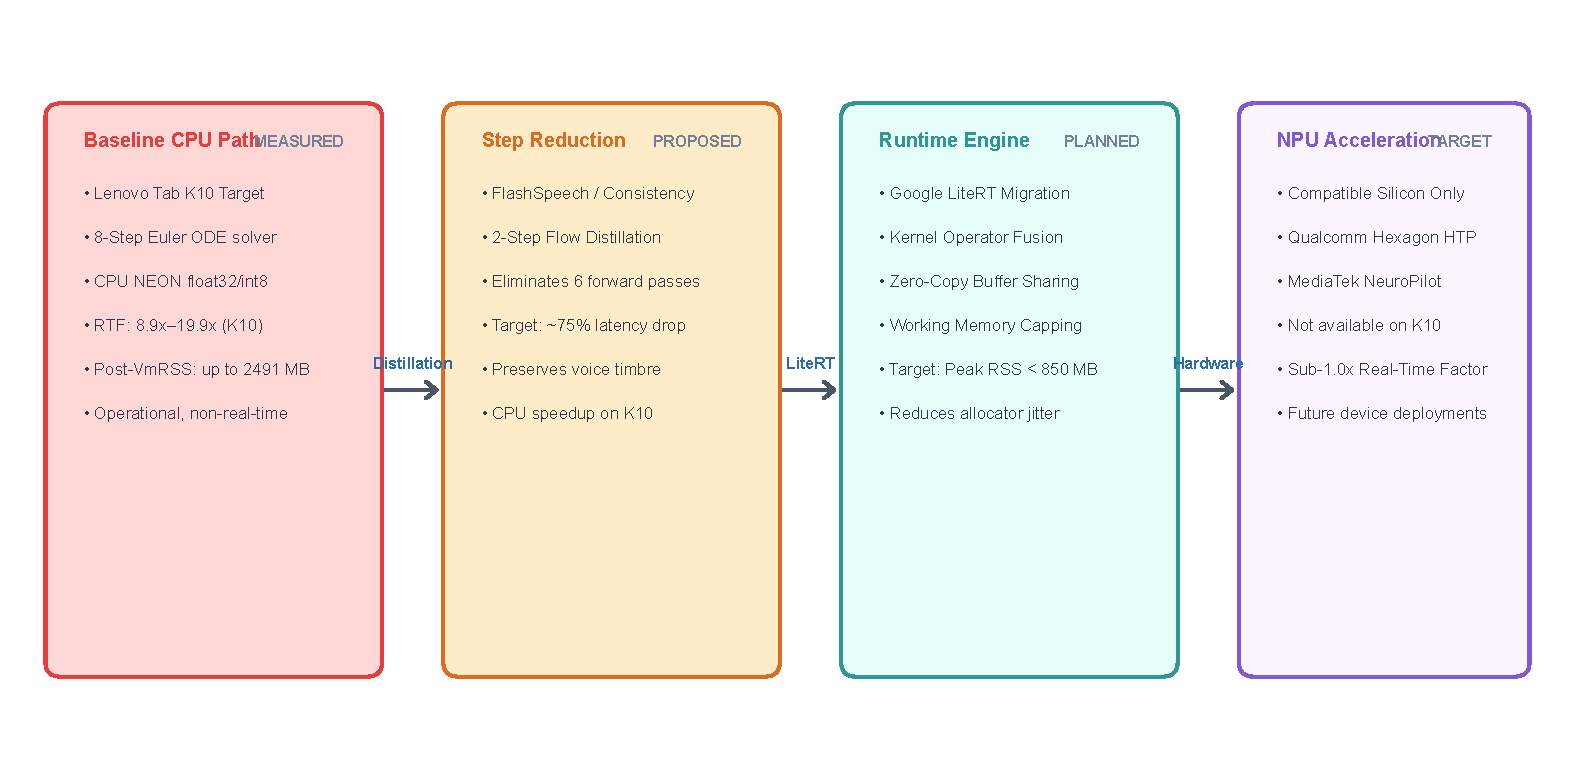
\includegraphics[width=0.92\textwidth]{Figures/optimization_roadmap.pdf}
\caption[Strategic Edge Acceleration and Optimization Roadmap]{Strategic edge acceleration roadmap, contrasting baseline CPU-only execution with operator fusion, step distillation, and hardware delegate acceleration paths.}
\label{fig:optimization_roadmap}
\end{figure}

\begin{table}[htbp]
\centering
\caption[Architecture Comparison: ONNX Runtime vs. Google LiteRT]{System Architecture Comparison: Custom ONNX Runtime vs. Google LiteRT}
\label{tab:litert_vs_ort_comparison}
\resizebox{\textwidth}{!}{%
\begin{tabular}{lcc}
\toprule
\textbf{Architectural Dimension} & \textbf{Custom ONNX Runtime (C++)} & \textbf{Google LiteRT (LiteRT Torch)} \\
\midrule
Model Ingestion Path & PyTorch $\to$ ONNX $\to$ ORT & Direct PyTorch $\to$ \texttt{.tflite} FlatBuffer \\
Graph Operator Dialect & Generic ONNX standard & Optimized TFLite / StableHLO dialect \\
Transpose-Op Overhead & High (Frequent Transpose nodes) & Low (Fused native tensor layouts) \\
Snapdragon NPU Acceleration & Manual QNN Execution Provider & Native Qualcomm AI Engine Direct \\
MediaTek APU Acceleration & Unstable Android NNAPI fallback & Native MediaTek NeuroPilot integration \\
Buffer Allocation & Custom heap memory arenas & Zero-copy Android Hardware Buffers \\
Runtime Binary Footprint & Heavy (>75\,MB \texttt{.so} dependencies) & Lightweight (~8--12\,MB runtime) \\
Ecosystem Integration & Manual NDK CMake \& Dart FFI & Google Play On-Device AI (PODAI) \\
\bottomrule
\end{tabular}%
}
\end{table}

\section{Direct PyTorch Conversion via LiteRT Torch (\texttt{litert-torch})}
Historically, converting PyTorch generative models to TensorFlow Lite required exporting to ONNX, followed by conversion via \texttt{onnx2tf} or \texttt{tf2onnx}, an error-prone multi-stage process that frequently failed on dynamic shapes or custom attention kernels.

The modern LiteRT toolchain introduces \textbf{LiteRT Torch} (\texttt{litert-torch})~\cite{litert_torch2024}, enabling direct compilation from native PyTorch code into optimized \texttt{.tflite} FlatBuffers:

\begin{lstlisting}[language=Python,caption={Conceptual PyTorch-to-LiteRT Conversion Pipeline via litert-torch}]
import torch
import litert_torch

# 1. Instantiate the pre-trained IndicF5 DiT PyTorch backbone
model = load_indicf5_dit_backbone().eval()

# 2. Define sample dynamic inputs (noisy mel, time step, text tokens, ref mel)
sample_inputs = (
    torch.randn(1, 100, 512, dtype=torch.float32),   # x_t
    torch.tensor([0.5], dtype=torch.float32),         # time step t
    torch.randint(0, 187, (1, 64), dtype=torch.int32),# text tokens
    torch.randn(1, 100, 350, dtype=torch.float32),   # ref mel conditioning
)

# 3. Export model graph using PyTorch 2.x export infrastructure
exported_program = torch.export.export(model, sample_inputs)

# 4. Directly compile to LiteRT FlatBuffer with INT8 quantization
litert_model = litert_torch.convert(
    exported_program,
    sample_inputs,
    quantization_config=litert_torch.QuantizationConfig.int8_ptq()
)

# 5. Serialize FlatBuffer to disk
litert_model.save("models/indicf5/indicf5_dit_int8.tflite")
\end{lstlisting}

\subsection{StableHLO Dialect and Operator Fusion}
LiteRT Torch translates PyTorch operators into \textit{StableHLO} (Stable High-Level Optimizer) intermediate representations. Within the StableHLO dialect:
\begin{itemize}
    \item Multi-head self-attention projections ($\mathbf{Q}, \mathbf{K}, \mathbf{V}$ linear layers) are fused into batched matrix contractions.
    \item Rotary Position Embedding rotations (\eref{eq:rope_rotation}) are fused with attention dot-product kernels, eliminating redundant intermediate tensor allocations.
    \item Layer normalization and ConvNeXt depthwise convolutions are transformed into optimized SIMD primitives.
\end{itemize}

\section{Hardware Acceleration via the CompiledModel API}
A key capability of Google LiteRT is the \textbf{\texttt{CompiledModel} API}, which abstracts low-level vendor delegates behind a unified declarative interface.

\subsection{Declarative Accelerator Prioritization}
In Android edge applications, the developer specifies a hardware execution hierarchy. The runtime automatically probes the underlying silicon, binds to available vendor drivers, and falls back gracefully if hardware acceleration is unavailable:

\begin{lstlisting}[language=Java,caption={Kotlin/Android CompiledModel Initialization with Accelerator Priority}]
import com.google.ai.edge.litert.CompiledModel
import com.google.ai.edge.litert.Accelerator

val options = CompiledModel.Options().apply {
    // Set hierarchical accelerator priority: NPU -> GPU -> CPU
    setAcceleratorPriority(listOf(
        Accelerator.NPU,
        Accelerator.GPU,
        Accelerator.CPU
    ))
    setNumThreads(4) // 4 threads for XNNPACK CPU fallback
}

// Compile model ahead-of-time or on-device
val compiledModel = CompiledModel.create(
    context.assets.openFd("indicf5_dit_int8.tflite"),
    options
)
\end{lstlisting}

\subsection{Qualcomm AI Engine Direct (QNN) Integration on Compatible Silicon}
When running on compatible devices powered by Qualcomm Snapdragon platforms (such as the Samsung Galaxy S23 featuring the Snapdragon 8 Gen 2):
\begin{itemize}
    \item LiteRT binds directly to Qualcomm AI Engine Direct (QNN)~\cite{qualcomm_qnn2024}.
    \item Matrix multiplications in the DiT layers are offloaded to the Hexagon Tensor Processor (HTP), executing 8-bit integer dot products with dedicated hardware vector units.
    \item This hardware offloading is targeted to substantially reduce per-step evaluation latency compared to CPU execution, establishing an analytical throughput design target below $0.5\times$ RTF for compatible flagship silicon.
\end{itemize}

\subsection{MediaTek Silicon Considerations and CPU-Side Optimization on Budget Platforms}
For MediaTek platforms, hardware support diverges sharply based on chipset tier:
\begin{itemize}
    \item \textbf{Mid-Range and Premium Dimensity SoCs}: On newer Dimensity platforms equipped with dedicated APUs, LiteRT offloads supported quantized operators via MediaTek NeuroPilot~\cite{mediatek_neuropilot2024}.
    \item \textbf{Target Budget Hardware (Lenovo Tab K10)}: The MediaTek Helio P22T chipset lacks an on-chip Neural Processing Unit or dedicated deep learning accelerator. Consequently, neither Qualcomm QNN nor MediaTek NeuroPilot can accelerate the K10. On this hardware class, LiteRT automatically engages the XNNPACK engine, executing optimized 4-thread ARMv8 NEON assembly routines.
    \item \textbf{Targeted CPU-Side Enhancements for Budget Hardware}: For devices like the Tab K10, performance gains must be achieved purely through CPU-side optimizations:
    \begin{enumerate}[label=(\alph*)]
        \item Algorithmic sampling step reduction (distilling 8 Euler steps down to 2 or 4 steps);
        \item Pre-allocated static tensor arena reuse to eliminate dynamic memory allocations;
        \item StableHLO operator fusion to minimize intermediate tensor bandwidth; and
        \item Warm runtime session retention to eliminate cold-start reinitialization overhead.
    \end{enumerate}
\end{itemize}

\section{Zero-Copy Pipelines via Android Hardware Buffers}
In traditional deep learning runtimes, passing generated mel-spectrogram tensors from the acoustic model to the neural vocoder and subsequently to the audio output track incurs memory copying overhead:
\begin{equation}
    \text{Model Heap} \xrightarrow{\text{memcpy}} \text{Vocoder Input Buffer} \xrightarrow{\text{memcpy}} \text{PCM Audio Track}
\end{equation}
On memory-bandwidth-constrained edge SoCs, these copies generate memory bus stalls and inflate physical \acrshort{rss}.

LiteRT addresses this via native support for \textbf{Android Hardware Buffers} (\texttt{AHardwareBuffer}):
\begin{enumerate}
    \item The output tensor of the DiT model and the input tensor of the Vocos vocoder are allocated in a shared, memory-mapped \texttt{AHardwareBuffer}.
    \item The Fourier Inverse STFT synthesis is performed in-place within this memory-mapped hardware buffer.
    \item Synthesized PCM audio samples are streamed directly to the Android low-latency audio subsystem (AAudio / OpenSL ES) without intermediate user-space buffer duplication.
\end{enumerate}

\section{Trajectory Distillation: 2-Step and 4-Step Sampling}
While hardware acceleration reduces per-step evaluation latency, algorithmic acceleration reduces the total number of steps required to solve the continuous flow-matching ODE. As established in \cref{Chapter2}, our post-midsem roadmap incorporates two distinct trajectory distillation techniques:

\subsection{Rectified Flow Trajectory Straightening (4-Step Reflow)}
By retraining the IndicF5 DiT model on synthetic coupled pairs $(\mathbf{x}_0, \mathbf{z}_1)$ generated by the base 1-rectified model (\eref{eq:reflow_loss}), trajectory crossing is eliminated. In 2-rectified flow, the vector field paths become straight lines, allowing a 4-step Euler solver to achieve Mean Opinion Scores comparable to the 8-step baseline, cutting overall computational requirements in half.

\subsection{Consistency Distillation and Few-Step Trajectory Solving}
Adapting consistency distillation principles~\cite{flashspeech2024} to the flow-matching framework trains a student network to map any point along an ODE trajectory directly to the origin data point while enforcing boundary condition self-consistency:
\begin{equation}
    f_\theta(\mathbf{x}_{t_1}, t_1) = f_\theta(\mathbf{x}_{t_2}, t_2) \quad \forall \; t_1, t_2 \in [0, 1]
\end{equation}
By learning to traverse large temporal intervals in single evaluations, consistency distillation enables generating candidate mel spectrograms in two sampling steps. Rather than assigning arbitrary physical roles to individual numerical steps, few-step consistency models evaluate the trajectory vector across broad time horizons ($t \in [0.0, 0.5]$ and $t \in [0.5, 1.0]$), progressively refining the acoustic canvas toward target spectral densities.

Executing two steps rather than eight reduces total computational cycles on mobile ARM cores by up to 75\%. However, few-step distillation can introduce trade-offs in fine phonetic naturalness or spectral detail, making post-midsem perceptual listening tests and objective intelligibility evaluations essential before deploying two-step checkpoints into production classrooms.

\section{Physical Testing and Verification Protocol}
The post-midsem implementation will be validated against a standardized physical testing protocol across our target device tiers:

\begin{enumerate}
    \item \textbf{Phase A: Graph Compilation and Validation}:
    \begin{itemize}
        \item Validate numerical parity between PyTorch FP32 outputs and LiteRT INT8 \texttt{.tflite} outputs (evaluating objective speech similarity and spectral distortion).
        \item Verify that INT8 quantization introduces minimal perceptual degradation across Vocos iSTFT reconstructions.
    \end{itemize}
    
    \item \textbf{Phase B: Ahead-of-Time Acceleration Profiling}:
    \begin{itemize}
        \item Measure per-operator execution times on Qualcomm QNN HTP (Galaxy S23) and MediaTek NeuroPilot (on compatible Dimensity platforms).
        \item Verify delegate coverage across DiT layers and Vocos ConvNeXt blocks, tracking any fallback to CPU execution.
    \end{itemize}
    
    \item \textbf{Phase C: Real-World Battery, Thermal, and Memory Benchmarking}:
    \begin{itemize}
        \item Continuously synthesize sentences from \texttt{prompts.json} to monitor thermal throttling curves and battery consumption.
        \item Continuously profile \texttt{/proc/self/status} (\texttt{VmRSS}) on the Lenovo Tab K10 to evaluate whether resident memory stabilizes within our analytical 801\,MB budget envelope under sustained multi-sentence operation.
    \end{itemize}
\end{enumerate}
